\chapter{Designing and Building the System} \label{development}  

The goal of this thesis is to evaluate the suitability of Blockchain technology
in managing the identity of patients in an Healthcare organization by
conceptualizing and implementing a system that fulfills this role. In order to
fulfill this goal, the development part of this thesis was primarily divided
into four steps with each step building upon the previous ones. This Chapter
provides an insight into the workflow used to build the system. The workflow
spans the conceptualization and its associated challenges and ends in the
implementation of said system. This system was built using some of the
technologies and concepts described in the previous section.

\section{First Step - Defining Requirements and Choosing a 
	Platform}\label{choosingHyperledger}

After investigating the various Blockchain platforms some criteria was needed
to serve as reference. As such, the first step consisted in defining a set of
key points that the built system had to fulfill. Defining the requirements
proved helpful to choose the most appropriate platform for the objectives as
explained later.

\subsection{Requirement Definition}
The requirements for this work were deemed to be as follows:

\renewcommand{\labelenumi}{\Roman{enumi}.}
\begin{enumerate}
  \item The system must allow a patient to opt into the network and register as
    a participant.
  \item The system must allow a patient to record his medical data under the
    approval of an administrator.
  \item The system must keep information confidential, transparent and have
    high availability.
  \item The system must provide the patient with the ability to share his data
    with another entity participating in the network, for example sharing
    information with a doctor.
  \item The system must allow the deletion of a patient's data in some manner,
    if he wishes to do so, in order to comply with European privacy laws.
\end{enumerate}

These requirements were chosen in order to create a system that is interesting
to an organization while still respecting the patients data and their access
right to it. 

After defining the requirements it was nececessary to choose the Blockchain
platform that best fulfills these requirements.


\subsection{Choosing a Platform}\label{choosePlatform}

Even tough Blockchain platforms normally originate from the realization that
full centralization has major drawbacks they often have different goals
translating in architecture differences and different development focus.  These
range from open networks, such as Ethereum which anyone can join and use, to
permissioned distributed ledgers, which can be run publicly or privately but
are only open to access and participation through a membership service, such as
Hyperledger Fabric and Hyperledger Indy.

Ethereum is a popular platform on its own right and has certainly paved the way
for Blockchain to be used as a platform that can be extended and built upon. It
has a growing learning ecosystem and community. It is easy to start interacting
with the network as anyone is able to simply download a client and connect to
it.  Thanks to the Solidity smart contract language being targeted for the
specific purpose of authoring smart contracts it only allows for a
deterministic program to be written avoiding potential conflicts in the
execution of these, for example, in the production network. Also after the
initial learning barrier of it being a \textbf{dsl} it becomes a platform easy
to develop for since it provides a well thought out and well organized
documentation with a easy to use library of operations.

Ethereum is being used in a great deal of projects around the world proving its
stability and suitability in a wide variety of use cases. On the other hand,
handling patients medical data is a great responsibility due to the private and
personal nature of this data. Also hospitals and Healthcare clinics must obey
the regulatory laws regarding privacy and usage of this data.

It is also worth noting that while Ethereum can handle private data exchange by
building upon it, as shown by Barclay, it was not designed with this intent in
mind, therefore these middle ground solutions can prove to be unwise to use at
scale given Ethereum's and the whole Blockchain's ecosystem past problems with
scalability.  

Fabric, like Ethereum, was built with the intention of being a general purpose
use Blockchain. It provides developers with the tools needed to build any
system they can imagine. However, the latter is clearly focused on making
organizations feel more at ease by being auditable as it offers an identity
service and a known environment due to using a membership service provider,
using a private certificate authority that emits certificates specific for the
Fabric network. These concerns allow this platform to avoid the same fate as
\textbf{IoT} devices have had in the Healthcare field~\cite{Tana2017}. The lack
of security regulations and ambiguity in how data was being collected by these
devices has limited their usage and prevented the widespread usage of these
devices in the Healthcare field.

Fabric also has good amount of development tools that are now maturing and a
good learning environment with ample documentation about every aspect important
for a developer looking to get started into it. Fabric is being backed by the
Linux Foundation and IBM, lending credibility to the project and ensuring that
this platform is supported and developed into the foreseeable future, as it is
being governed by a diverse technical steering committee and by a diverse set
of maintainers from multiple organizations. In regards to performance the focus
in this area is clear as the Hyperledger community has appointed a Performance
and Scale working group to improve performance as well being tasked to
implement benchmarking framework for Hyperledger projects called Hyperledger
Caliper~\cite{performanceScale2017}.

Regarding Fabric's features, it lends itself very well to fulfill the project
requirements. Fabric's channels and private data segregation at peer level make
a clear statement that privacy is important in this platform which is in line
with the requirements that were laid out for this project. It is also worth
noting that many upcoming Blockchain based projects in the Healthcare field are
using permissioned networks due to these same concerns regarding the privacy of
the patients while retaining the key benefits of Blockchain such as
immutability and decentralization. The fact that Fabric has no associated
currency also means there is no required mining incentives to maintain the
network, even tough it does require some additional infrastructure acquisitions
to set up the network, leading to a higher initial investment in a solution
based on this platform.

Both are very interesting platforms, but ultimately it was decided to use
Hyperledger Fabric as the platform on which to build upon. This decision was
taken in part because Fabric was purpose built for a very regulated environment
and is focused on privacy and scalability which are required in the Healthcare
field. Also, this technology is relatively recent and there is still a great
lack of knowledge available to the general public, making it a more interesting
choice from an theoretical standpoint.


\section{Working knowledge of the Platform}

After choosing to work with Hyperledger Fabric it became necessary to
understand in further detail what are the components that form a network and
the tools to manage these components. This section discusses the main
components of a Fabric network and the tools required to create and maintain a
Fabric network. These components often interact with one another and provide
the technical infrastructure that comprises this technology.

\subsection{Hyperledger Fabric Components}

An Hyperledger Fabric (HLF) network is defined as the technical infrastructure
that provides ledger and smart contract services to applications. Smart
contracts are used to generate transactions and interact with the ledger. The
network is comprised of several components as presented shortly.

The ledger is a central component of a HLF network. The ledger is composed by a
world state and a Blockchain. The world state is a database that holds the
current values of ledger states. States are, by default, expressed as key-value
pairs. The world state is useful because it makes it easy for a smart contract
to get the current value of these states, instead of having to traverse the
entire transaction log. The Blockchain holds the transaction logs that record
the history of changes that have resulted in the current world state.
Transactions are collected and recorded in an immutable sequence of blocks, in
which each block contains a set of ordered transactions by the orderer service.

Another component is the set of peers participating in the network. A Peer is a
node that hosts a copy of the multiple ledgers and smart contracts. There is
one logical ledger in a Hyperledger Fabric network, even tough in reality, the
network maintains multiple copies of a ledger that are synchronized through
consensus. HLF opts to allow multiple ledgers in a network to achieve different
goals of a greater purpose. This allows the creation of channels of information
between trusted parties, for example, a channel of secure and private
information between the clinical staff of an hospital and a patient as
discussed on Chapter~\ref{background}, in which every channel has a ledger.

Through a peer connection, applications execute chaincode that queries or
updates a ledger. Peers have at least one of the three different roles assigned
to them, as seen on Section~\ref{distributedLedgerPlatform}. Applications
always connect to peers when they need to access ledgers and smart contracts.
Every peer in the network is assigned a digital certificate by an administrator
from its owning organization. The mapping of a peer's identity in an
organization is provided through the membership service provider. 

In fact peers, applications, end users (clients), administrators, channels and
organizations must have an identity provided by the MSP in order to be able to
interact with the network. Each of these actors has a digital identity
encapsulated in an X.509 digital certificate standard which must be unique to
every entity. These determine the exact permissions these have over resources
and access to information in the network. The MSP issues these certificates
through the built-in CA component, the Fabric Certificate Authority (CA). The
Fabric CA is a private root CA provider that consists in a CA server and a CA
client. The MSP also supports Certificate Revocation Lists (CRL).

\subsection{Administrating a HLF Networks}


As discussed, a HLF network must have an administrator. HLF provides the
\textit{cryptogen}, \textit{configtxgen}, \textit{configtxlator} and
\textit{peer} tools that are used to configure the network to suit different
needs and use cases.

The \textit{cryptogen} tool generates cryptographic data consuming the file
\textit{crypto-config.yaml}.

The \textit{configtxgen} tool generates the genesis block for the orderer
services and the initial transactions.  This tool consumes the file
\textit{configtx.yaml} that defines configuration parameters for channels, the
genesis block and the orderer service.

The \textit{configtxlator} tool is also used to generate channel
configurations.  Finally the \textit{peer} tool is used to manage the
participating peers in the HLF network.

These tools are used to create and maintain the topology of the network and are
invoked when a change to the network is made, for example, when permissions to
certain records are changed or a new user is enrolled in the network and are
very much intertwined with the Fabric Certificate Authority (CA) discussed in
subsection .

\section{Building the System}

After considering the project goals of investigating the suitability of a
Blockchain based system to manage patients in Healthcare, the third step was to
build a prototype of a system that would provide a simulation of the production
network, albeit on a smaller scale. The insights gained from developing a
simple working system would enable benefits and risks of the approach to be
identified, and opportunities for further research to be laid out.

In order to build a solution, the research done before hand was taken into
account and allowed a global overview of how architecturally a system could be
built with the components available. After some consideration some approaches
were reached and are now presented.

\subsection{Conceptualization and Design}

After some thought it was determined that the information that defines the
patient's identity is a key requirement to build a system that recognizes
patients across the Healthcare environment, as discussed in
Chapter~\ref{background}. An asset could be created through chaincode that
represents the concept of the patient's identity in this network. An asset is
stored in a Fabric network as a key-value pair. The key for this kind of asset
could be a string. The string could be composed by the string 'Patient\_'
followed by a patient identification number assigned when the data is entered
into the Blockchain. Since optimization is not a key concern to build a simple
prototype in this thesis context, the patient's identification number was
defined to simply be the order of the data entry starting at number one. This
ensures that the key is unique and it is easily computable. In short, it was
decided that the key is formed by the string 'Patient\_' followed by the
mentioned patient identification number. This key is used to query and access
information of a patient.

To aid in interoperability with other systems, as seen in Figure
\ref{fig:interoperability}, the Fast Healthcare Interoperability Resources
(FHIR) standard by the Health Level 7 organization could be used as basis for
the fields in the structure used to represent the patient's identity in the
Healthcare domain.  Each field of the patient's identity structure, defined in
a smart contract, would be linked to a field of the
\href{http://www.hl7.org/fhir/patient.html}{patient structure as presented in
the FHIR standard}.

\begin{figure}[ht] \centering
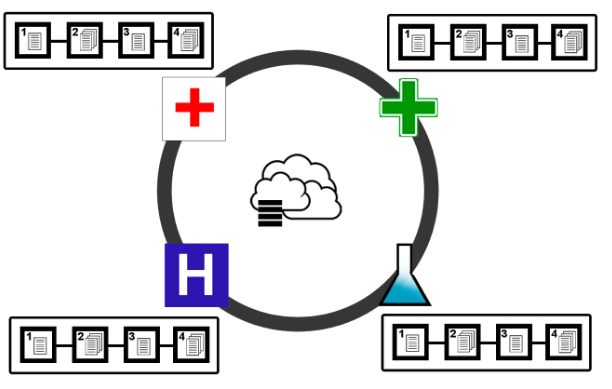
\includegraphics[width=0.7\linewidth]{imgs/interoperability.png}
\caption{\label{fig:interoperability}An Example of Interoperability with the
Blockchain Network} \end{figure}

The most simple case of an interaction in an Healthcare service is the
interaction between a patient and a doctor. In HLF this situation translates to
two organizations and two peers. Each peer belongs to an organization. One
organization represents the patients while the other represents the hospital
where the doctor works. 

To establish a communication between the two participating peers a channel can
be created ensuring information exchanged between the two on the channel is
private and does not exist on the rest of the network.  If a third organization
with another peer representing another health clinic joined the network then
another channel could be created between the patient's organization and this
new organization. If the patient were to insert his data into the channel then
the clinic would be able to view it everytime they wished. 

Starting in version 1.1 of Fabric the MSP allows Attribute Based Access Control
meaning access flow to the data can depend on the value of a certain attribute
of the certificate. Also it is possible to encrypt data and insert it into the
channel and then require a key to decrypt the data. In this case the patient
could give a key to the doctor to be able to access only his data. In the
current version of Fabric, version 1.2, private data collections were
introduced, meaning that some data can be marked as private on a channel while
other data can be public.

To conclude it was tought that to properly evaluate this solution a series of
experiments would be conducted. First some data would be present on the channel
when the user interacts that represents his identity in a certain clinic. The
patient would query the Blockchain for his data and receive his data if
everything worked accordingly. The second experiment was making the patient
share his data with the doctor in the channel. The last experiment consisted in
the patient trying to query data of another patient that was inserted at the
genesis of the network and seeing if the data was encrypted or was easily
readable. The outcomes of these experiments can shape the development of the
solution as it could take these results into consideration and highlight
possible problems.


\subsection{Implementation}

To create an interactive system that can manage the patients identity in an
Healthcare environment an application was built that the user interacts with.
Applications can be developed in any language as long as there is a Software
Development Kit (SDK) supporting the language. 

At the time of writing there is the Go language SDK and Node.js SDK available
with Go being the first programming language to get support and Java also being
added recently. 

After some research the Node.js SDK seemed to be on par with the Go one, in
regards to API and features. However, documentation was more sparse and harder
to find for the Node.js SDK. 

On the other hand Javascript seemed more approachable in contrast to Go, in
order to implement the system due to the author's familiarity with the Node.js
environment and with the Javascript programming language. Also, the application
and the smart contract could both be built in this language which was
considered an advantage as it simplifies dependency management. 

Ultimately, this application interfaces with smart contracts through the
Hyperledger Fabric Software Development Kit and the chaincode was built using
the Hyperledger Fabric Shim for Node.js and programmed in Javascript.

To avoid the need for multiple machines being used to form the network, a
Docker Compose file was used that defines, and orchestrates the main components
of the network through the Docker Engine. Each component consists in one or
more containers. Also, there is one  container defined to be used as a CLI to
interface with the network using the peer tool if needed for administrative
purposes. Docker was used as the containerization technology because it is
officially supported by Hyperledger and is currently the most popular
containerization tool.

To build the desired network configuration for the prototype, the configuration
file for the \textit{cryptogen} tool was edited to allow the network to have
two organizations, each of them with a peer associated. The configuration file
for the configtxgen tool was also edited to allow a channel of information
between the two organizations to be created. Each peer would serve as the
anchor peer~\footnote{Used to initiate communication between peers from
different organizations. The anchor peer serves as the entry point for another
organization’s peer on the same channel to communicate with each of the peers
in the anchor peer’s organization.} in each of the organizations.

An application was also built that allows for user enrollment to create a new
identity in the network. The application is run by a user and uses the
available SDK to call upon the operations that the smart contract makes
available. When a new user of the application enters the network, a function in
the smart contract initializes the creation of the patient's data and writes
the patient's Healthcare information to the ledger as a new asset and also
manages the ledger state through transactions as well as the world state.  The
overview of the architecture for this system is represented on Figure
\ref{fig:appOverview}. Due to the security mechanisms these transactions are
signed and endorsed by the administrator of the network and verified by the CA
servers.

\begin{figure}[ht] \centering
  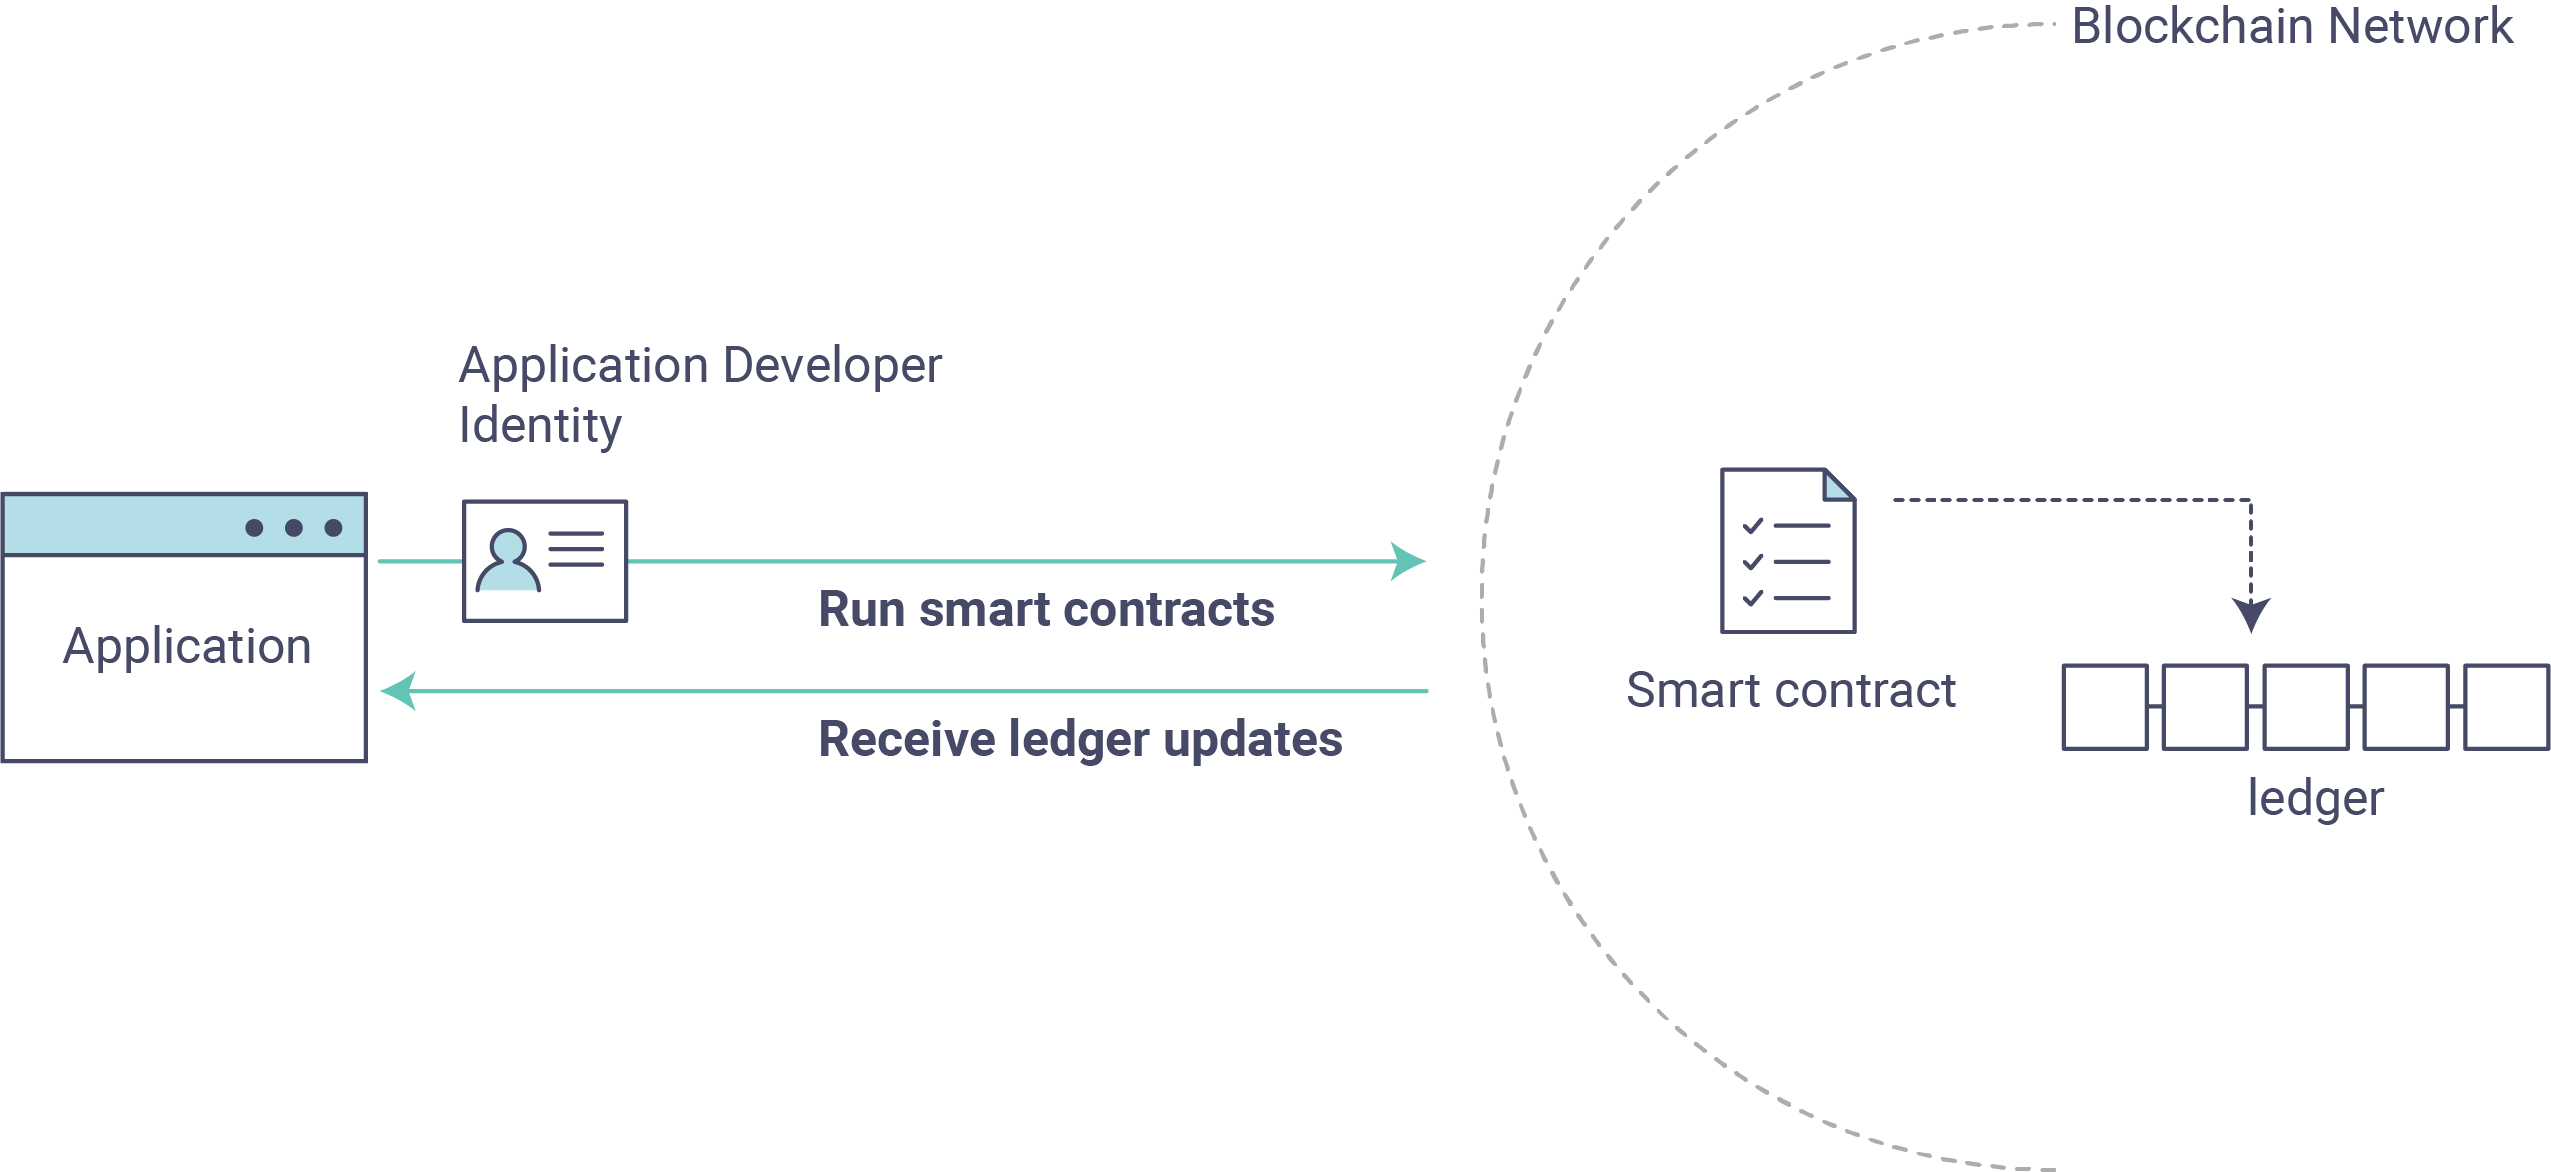
\includegraphics[width=1\linewidth]{imgs/hyperledgerAppOverview.png}
  \caption{\label{fig:appOverview}An Overview of the System Architecture
  (Source:
  \href{http://hyperledger-fabric.readthedocs.io/en/latest/write_first_app.html}{HLF
  Fabric Documentation})} 
\end{figure}

The assets loaded contain the necessary fields to identify a patient in an
Healthcare context, such as its name and birth date, for example, as well as
some other information necessary to manage this data as discussed previously.


These operations form an Application Programming Interface (API) as seen in
Figure \ref{fig:smartContractOverview} that returns a payload in JSON format
with information from the network. This API allows a query to be made to the
network that returns the patients information, changing incorrect or outdated
information or disabling the identity structure of someone who is not
participating in the network actively anymore in order for that information to
be read-only from that point on, for example, with more available. This system
architecture leads to a modular as well as extensible approach regarding the
availability of new operations that become available as soon as new versions of
the smart contract are deployed.  

\begin{figure}[ht] 
  \centering
  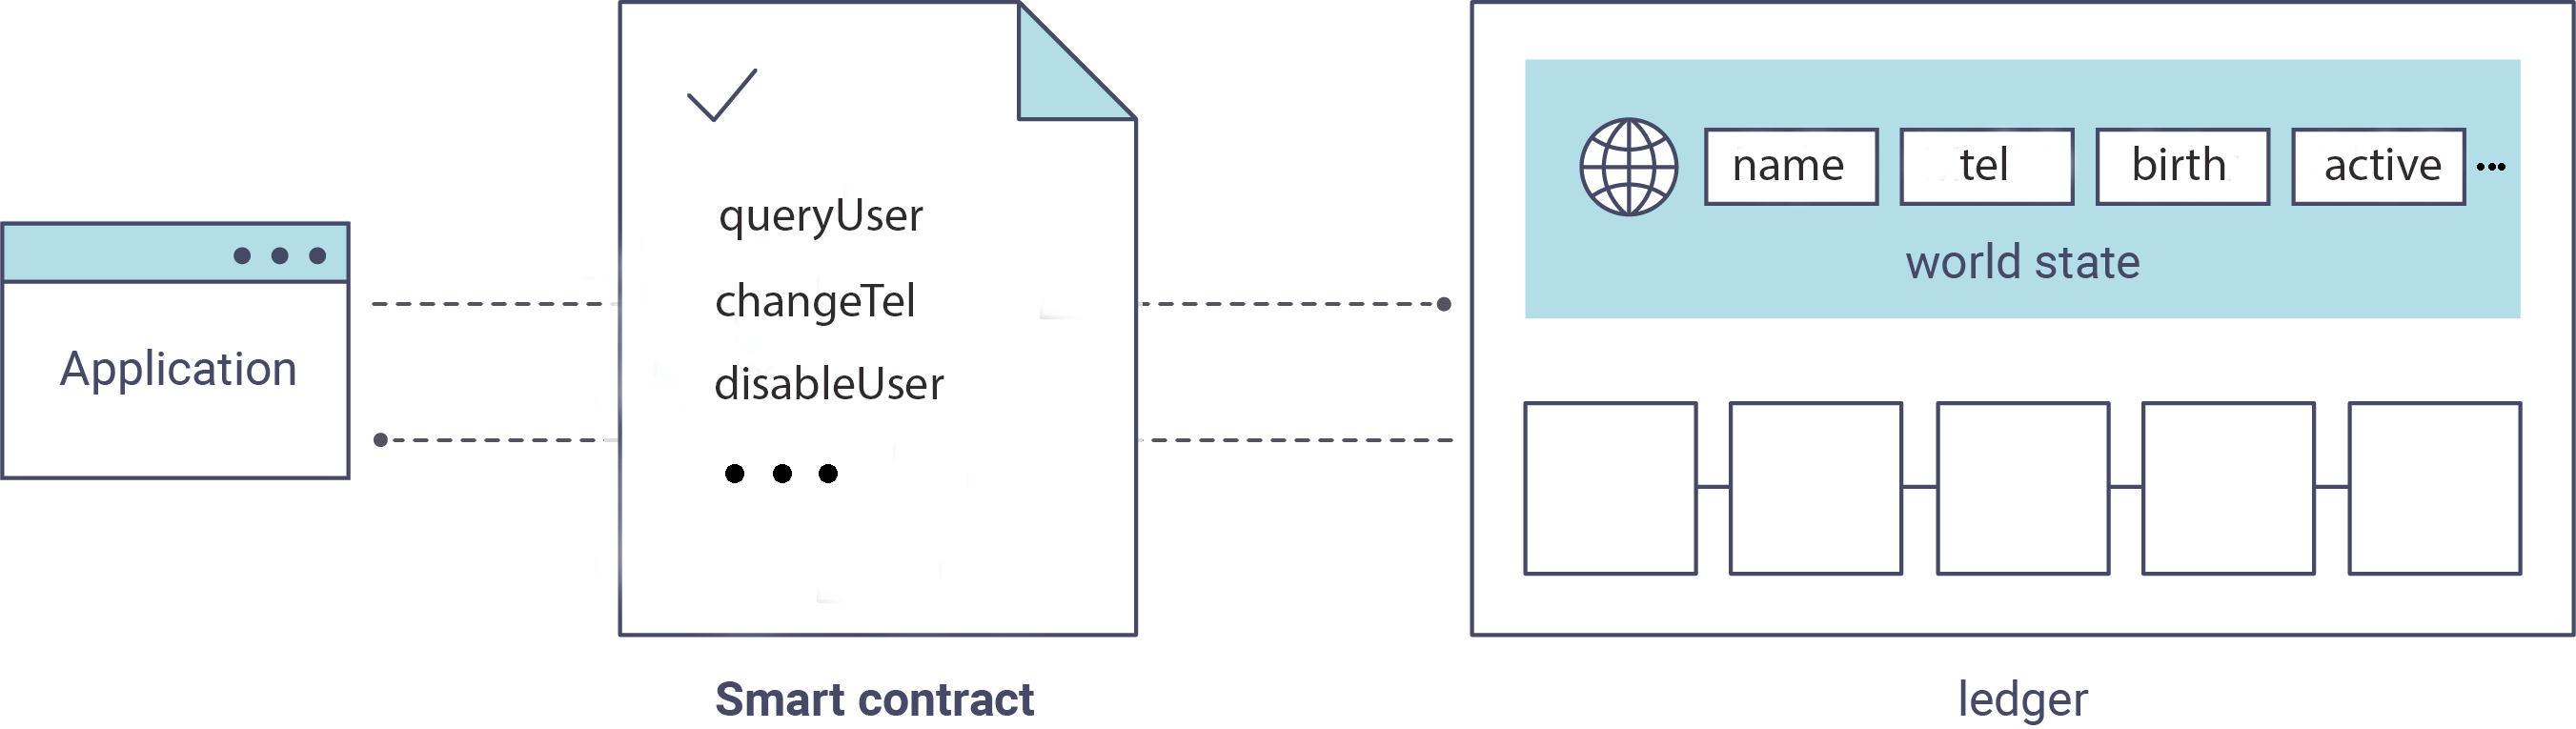
\includegraphics[width=1\linewidth]{imgs/smartContractOverview.png}
  \caption{\label{fig:smartContractOverview}Smart Contract Operations Example
  (Original:
  \href{http://hyperledger-fabric.readthedocs.io/en/latest/write_first_app.html}{HLF
  Fabric Documentation})} 
\end{figure}

The network was brought up using the Docker Compose technology and an
administrator was enrolled into the network. This step is required because
every action must be verified through a chain of trust and the administrator is
the root CA in the network.

The next step was registering the patient and the doctor. Both the patient and
the doctor ran the register function of the application and were asked for a
password. After successfully registering they were show their assigned patient
number and the password was stored in the certification as well as the patient
number assigned to them. At this point they became active participants in the
network. In this case the assets that represent their identity were not created
because they had exceptionally been created before hand by the administrator to
simplify the process. The normal flow would be the respective asset creation on
registration.

\section{Testing and Adjusting the System}

With the network in place and the peers set up and registered the experiments
proposed have now their requirements fulfilled.

\subsection{Experiments}

The patient used the function provided by the application to query the network
for his information. He searched for his patient number and was shown his
information successfully. This shows that the information was recorded with
success when the chaincode was deployed. The simple way to query personal
information with an assigned patient number also proved successful and shows
that this system can be used to store patient's identity data and retrieve it.

Then the patient had to share his information with the doctor. To do this it
was necessary to assume that the patient had given his patient number to the
doctor so that he could use the application built to query for that patient
number. The doctor queried the network for the patient's information and was
able to access it successfully. This proves that this platform allows
surprisingly, to very easily share information between a patient and a doctor
using a smart contract in a simple way.

Finally the patient tried to access another patient's data. It was necessary to
assume that he was given the patient number by the respective patient. When he
queried the network for that patient's data it became clear what already had
arose suspicions in the previous experiments. He was actually able to access
that data without a problem. This would be okay if the number was willingly
given to him. However if the number was obtained unwillingly it could prove a
problem. This meant that the solution currently, did not meet the requirement
of the information being confidential that was defined previously, even tough
it is transparent and has high availability since the information was spread
through multiple peers and could be on multiple channels. It became clear that
some additional data security measures was needed.

\subsection{Encrypting Data}

To make information confidential some form of obfuscation or encryption could
be used. Fabric also features Attribute Based Access Control meaning that the
chaincode logic could be altered to check if some attribute was present on the
doctor's certificate that indicated that he had access to certain patients
information. This could work for application users however if users used some
tool like Hyperledger Explorer they could see the data since the data is stored
as a plain text.

After investigating the different possibilities and making some tests it was
decided to use encryption. The flow of the operations would be simple. When the
patient's data was registered he would receive a notification of a data key and
the data would be encrypted using for example a traditional SHA-256 encryption
algorithm. The data would be encrypted using symmetric key encryption with the
generated key being stored on the X.509 securely.  If the patient wanted to
share his information with with someone he would give him the key and that
would allow him to decrypt the encrypted patient's data.  To complete this
system the key should expire after a certain amount of time and refresh itself.

With this system in place the last requirement was fulfilled and the system is
now considered to be reasonable for the purposes of this thesis. At this point
it is reasonable to evaluate this solution as an identity management platform
in the Healthcare context.

\section{Evaluation and a Review of Thesis Goals}

This solution was evaluated against the international standard for information
security known as the CIA triad model, in order to draw further conclusions and
evaluate how secure the built system is in regards to its information which is
a critical concern in this field. The three pillars that form this standard are
the preservation of the confidentiality, ensuring information integrity and
information availability.

\subsection{Confidentiality}

Confidentiality of the information stored in the network was considered a key
requirement when the requirements were presented. The Hyperledger Fabric was a
prime candidate for building the solution upon due to its focus on privacy and
a more enterprise approach to Blockchain development. While it offers many
features such as channels that truly do segregate information in a way that
many equivalent platforms cannot do at the moment it is also true that by
default data will be stored in plain text. 

To solve this problem it was necessary to implement data encryption on top of
the network using chaincode. This way even if someone was able to access the
underlying database or if someone used a tool like Hyperledger Explorer to
explore the network all it would see is encrypted data that would require a key
to encrypt. With these considerations in mind it, even tough there are a number
of aspects that define confidentiality it can be said that the built system
provides a confidential data storage.

\subsection{Integrity}

One of the key aspects of a Blockchain system is the immutability of data. This
means that once information is written it cannot be changed or erased. The
transaction logs assure that the specific version of that asset is recorded
permanently in the network. In order to comply with privacy regulations some
data can become only visible as an hash but it still remains there. Therefore
the integrity of data on this Blockchain platform and solution is also
preserved.

\subsection{Availability}

Even tough Fabric is a permissioned Distributed Ledger Platform and as such it
is administrated by an administrator it is also distributed and therefore
avoids having a single point of attack. By default it is more available than a
simple informational system that is centralized. In this aspect it can be said
the more the network scales, the more robust it becomes and therefore more
availability it provides as information redundancy also increases.

\subsection{Thesis Goals}

The goal of this thesis was to evaluate if a system could be built based on
Blockchain technology to manage the patients identity in the Healthcare
environment. Using Hyperledger Fabric a system was built that successfuly can
create, manage and delete patients data. Information can be shared in a secure
manner and interoperability eases organization into adopting this system. This
system provides benefits to the medical staff as well as the patients due to
transparency in how data is handled and secured.

However the costs of deploying this system in a production ready environment
would be higher compared to a more traditional approach. Since this system is
build upon a Permissioned Platform, machines to host the central services need
to be acquired and an administrator of the platform is necessary for the
necessary maintenance. As the network grows it would become more resilient and
additional servers could be used to expand the core availability of Blockchain
components.

There is also the question of scalability. Even tough a Permissioned Blockchain
is always faster in relation to a Permissionless variant it still is far from
matching the SIBS system form example. If this system was intended for global
use then additional approaches would need to be taken.

With this said the pace of development has been relatively fast with new
releases on a quarterly basis that focus on the issues of scalability and
privacy, two important features pertaining to the system this Thesis proposed.
